% Provenance (never printed): enseignement scientifique premiere (2019),
% theme "La Terre, un astre singulier: la forme de la Terre" (Eratosthenes,
% meridian measurement by triangulation, the metre); see
% sources/book2/PROVENANCE.md. Every length on the ellipsoid is computed in
% figdata/grade-10/meridian_degree.py (WGS 84, ledger wgs84:ellipsoid).
\chapter{Medindo a Terra}\label{ch:g10:measuring-the-earth}

Na praia, observe um navio que se afasta rumo ao mar aberto. Ele não
simplesmente encolhe até ficar pequeno demais para ser visto: primeiro
desaparece o casco, como se afundasse, depois a parte baixa da
superestrutura, e o topo do mastro some por último. O mar entre você e o
navio não é plano; ele se curva. Há mais de vinte e dois séculos, um sábio
de Alexandria transformou uma observação parecida --- o comprimento de uma
sombra ao meio-dia --- numa medida do tamanho do planeta inteiro. Este
capítulo acompanha essa medida e as que vieram depois: as cadeias de
triângulos que os agrimensores estenderam através de países inteiros, as
expedições enviadas ao Ártico e ao equador para saber se a Terra é
achatada, o nascimento do metro e os satélites com que o planeta é medido
hoje.

\begin{omfigure}
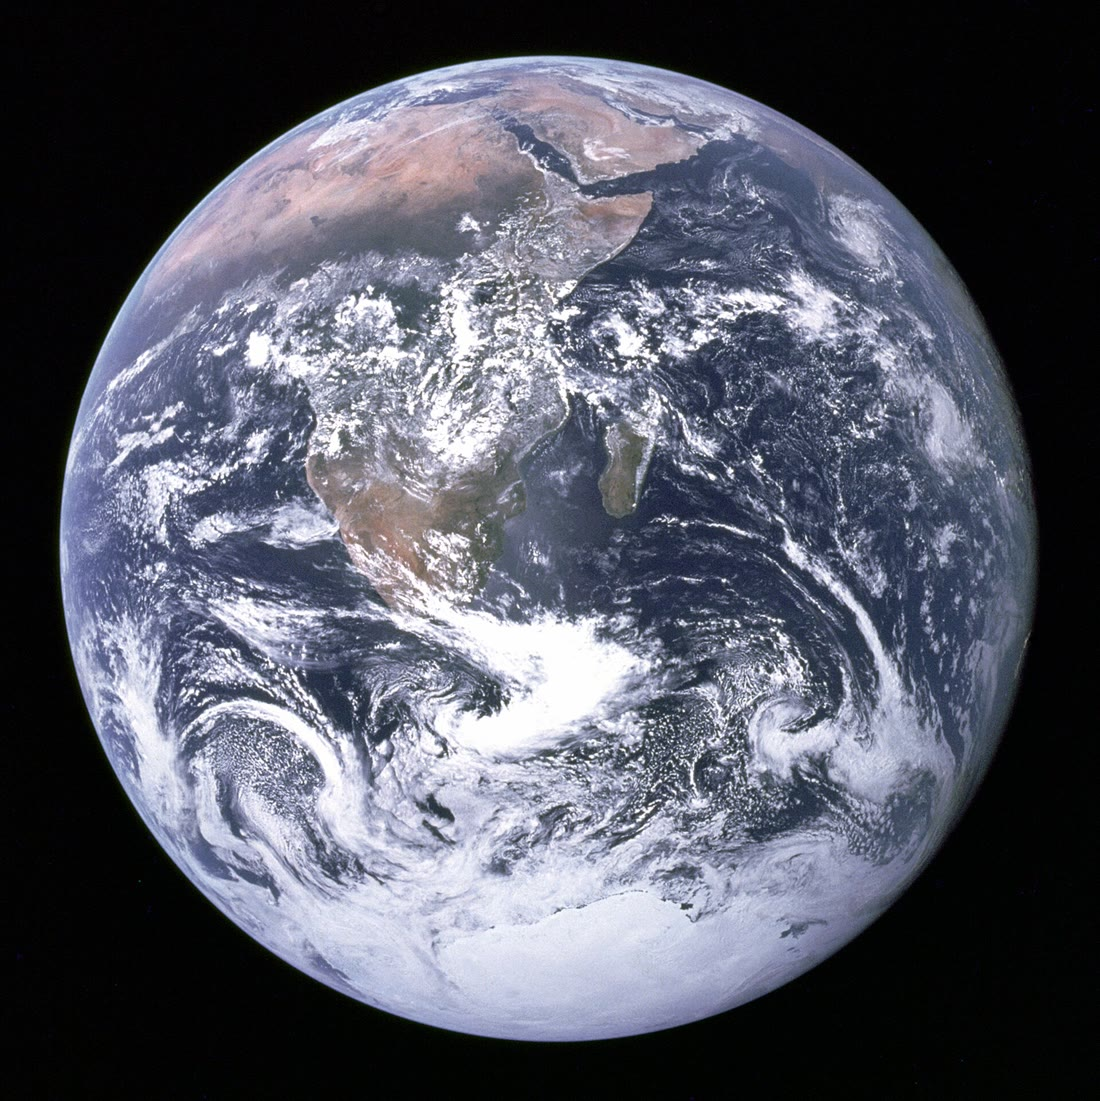
\includegraphics[width=0.5\linewidth]{images/book2/g10-nasa-apollo17-earth.jpg}

{\small A Terra fotografada pela tripulação da Apollo~17 a caminho da Lua,
em dezembro de 1972: a África, a Arábia e o gelo da Antártida. Fotografia:
NASA (domínio público).}
\end{omfigure}

\begin{recall}
Um lugar da Terra é localizado pela sua latitude, o ângulo ao norte ou ao
sul do equador, e pela sua longitude, o ângulo a leste ou a oeste de um
meridiano de referência; os meridianos ligam os polos, e os paralelos
contornam a Terra paralelamente ao equador (Livro 1). Num meio homogêneo, a
luz se propaga em linha reta, e os raios que chegam à Terra vindos do Sol,
muito distante, são paralelos (os livros de física). Num triângulo
retângulo, o seno de um ângulo agudo é o cateto oposto dividido pela
hipotenusa, o cosseno é o cateto adjacente dividido pela hipotenusa e a
tangente é o cateto oposto dividido pelo cateto adjacente (os livros de
matemática).
\end{recall}

\section{Uma Terra redonda}

Muito antes de alguém poder olhar a Terra do espaço, várias observações
mostravam que ela é redonda.
\begin{itemize}
  \item \textbf{Navios além do horizonte.} Um navio que se afasta
        desaparece de baixo para cima, em todas as direções e em todos os
        mares: a superfície do mar é curva em toda parte.
  \item \textbf{A sombra na Lua.} Durante um eclipse da Lua, a sombra da
        Terra cai sobre a Lua. A borda dela é sempre um arco de
        circunferência, qualquer que seja a hora da noite; só uma esfera
        projeta uma sombra redonda em todas as direções.
  \item \textbf{As estrelas mudam com a latitude.} Um viajante que segue
        para o norte vê a Estrela Polar subir mais alto acima do horizonte,
        e estrelas do céu austral desaparecem abaixo dele: o horizonte do
        viajante se inclina à medida que ele se desloca sobre uma
        superfície curva.
  \item \textbf{A volta ao mundo e a vista do espaço.} Navios, e depois
        aviões, deram a volta ao mundo em todas as direções; desde os anos
        1960, o planeta inteiro, redondo, é fotografado.
\end{itemize}

\begin{omfigure}
\begin{tikzpicture}[font=\small, >={Stealth[length=2.2mm]}]
  % sea surface: arc of a circle of radius 8 centred at (0,-8) (curvature exaggerated)
  \fill[omDef!10] plot[domain=-4.6:4.6, samples=60] (\x,{sqrt(64-\x*\x)-8}) -- (4.6,-2.2) -- (-4.6,-2.2) -- cycle;
  \draw[omDef!70!black, thick] plot[domain=-4.6:4.6, samples=60] (\x,{sqrt(64-\x*\x)-8});
  % observer on a small tower at x=-4 (surface y=-1.072), eye at y=-0.235
  \draw[black!70, line width=1pt] (-4,-1.072) -- (-4,-0.235);
  \fill (-4,-0.235) circle (2pt);
  \node[anchor=east, align=right] at (-4.1,-0.2) {olho do\\observador};
  % line of sight tangent at x=-0.5 (y=-0.0156, slope 0.0626)
  \draw[omThm!80!black, thick] (-4,-0.235) -- (4.4,0.290);
  \node[omThm!80!black, anchor=south, rotate=3.6] at (1.3,0.1) {linha de visada};
  \fill[omThm!80!black] (-0.5,-0.0156) circle (1.4pt);
  % ship at x=3 (surface y=-0.584), tilted 22 degrees with the local vertical
  \begin{scope}[shift={(3,-0.584)}, rotate=-22]
    \fill[black!12] (-0.6,0) -- (0.6,0) -- (0.75,0.32) -- (-0.75,0.32) -- cycle;
    \draw[black!45, densely dashed] (-0.6,0) -- (0.6,0) -- (0.75,0.32) -- (-0.75,0.32) -- cycle;
    \draw[black!45, densely dashed] (0,0.32) -- (0,0.95);
    \draw[black!80, line width=1pt] (0,0.95) -- (0,1.55);
    \fill[black!80] (0,1.55) -- (0.32,1.25) -- (0,1.25) -- cycle;
  \end{scope}
  \node[anchor=north, align=center, font=\footnotesize] at (2.9,-1.25) {casco e base do mastro\\escondidos pela curvatura};
  \node[anchor=north, font=\footnotesize] at (-0.5,-0.1) {horizonte};
\end{tikzpicture}

{\small Por que um navio desaparece de baixo para cima: o observador só vê o
que fica acima da linha de visada que tangencia o mar no horizonte. A
curvatura está muito exagerada.}
\end{omfigure}

\section{Eratóstenes mede a Terra}

Eratóstenes de Cirene (276--194 a.C.) era o bibliotecário de Alexandria.
Ele tinha ouvido dizer que em Siena, a atual Assuã, bem ao sul, subindo o
Nilo, o Sol iluminava todo o fundo de um poço ao meio-dia do dia do
solstício de verão: estava então exatamente a pino. Em Alexandria, no mesmo
momento, uma vara vertical projetava uma sombra curta: os raios do Sol
faziam com a vertical um ângulo de cerca de \qty{7.2}{\degree}, um
cinquenta avos de uma volta completa.
% ledger: erat:method, erat:stadion

\begin{omfigure}
\begin{tikzpicture}[font=\small, >={Stealth[length=2.2mm]}]
  \def\R{2.4}
  \fill[omDef!8] (0,0) circle (\R);
  \draw[omDef!70!black, thick] (0,0) circle (\R);
  \coordinate (O) at (0,0);
  \coordinate (S) at (\R,0);
  \coordinate (A) at ({\R*cos(25)},{\R*sin(25)});
  \coordinate (T) at ({(\R+0.75)*cos(25)},{(\R+0.75)*sin(25)});
  \coordinate (T2) at ({(\R+1.75)*cos(25)},{(\R+1.75)*sin(25)});
  % radii
  \draw[black!70] (O) -- (S);
  \draw[black!70] (O) -- (A);
  \draw[black!40, densely dashed] (A) -- (T2);
  \fill (O) circle (1.5pt) node[below left] {centro};
  % stick at Alexandria, along the radius
  \draw[line width=1.6pt, black!85] (A) -- ($(A)!0.6!(T)$);
  % well at Syene
  \draw[black!80, thick] ({\R-0.38},-0.12) -- (\R,-0.12) ($(S)+(0,0.12)$) -- ({\R-0.38},0.12);
  % parallel sun rays coming from the right
  \foreach \y in {-1.6,-0.8,0.8,1.6} \draw[->, omThm!70, thick] (6.6,\y) -- (4.4,\y);
  \draw[->, omThm!85!black, thick] (6.6,0) -- (\R+0.05,0);
  \draw[->, omThm!85!black, thick] (6.6,{(\R+0.45)*sin(25)}) -- ({(\R+0.45)*cos(25)+0.03},{(\R+0.45)*sin(25)});
  \node[omThm!85!black, align=center, anchor=west] at (4.6,2.35) {luz do Sol:\\raios paralelos};
  % angles
  \draw[omExo!80!black, thick] (0.75,0) arc (0:25:0.75);
  \node[omExo!80!black] at (1.05,0.22) {$\alpha$};
  \coordinate (Q) at ($(A)!0.6!(T)$);
  \draw[omExo!80!black, thick] ($(Q)+(0.8,0)$) arc (0:25:0.8);
  \node[omExo!80!black] at ($(Q)+({1.08*cos(12.5)},{1.08*sin(12.5)})$) {$\alpha$};
  \node[anchor=east] at ($(A)+(-0.12,0.18)$) {Alexandria};
  \node[anchor=north west] at ($(S)+(0.3,-0.12)$) {Siena};
  \node[font=\footnotesize, anchor=north] at ($(O)!0.5!(S)+(0.2,-0.05)$) {};
  \draw[<->, black!60] ({(\R-0.3)*cos(3)},{(\R-0.3)*sin(3)}) arc (3:22:{\R-0.3});
  \node[anchor=east, font=\footnotesize] at ({(\R-0.35)*cos(13)},{(\R-0.35)*sin(13)}) {$d$};
\end{tikzpicture}

{\small O raciocínio de Eratóstenes. Em Siena o Sol está a pino: seus raios
apontam para o centro da Terra. Em Alexandria, uma vara vertical, que também
aponta para o centro, faz um ângulo $\alpha$ com os raios. O ângulo no
centro entre os dois lugares é o mesmo $\alpha$. O ângulo está exagerado:
era de apenas \qty{7.2}{\degree}.}
\end{omfigure}

\begin{proposition}[Relação de Eratóstenes]\label{prop:g10:measuring-the-earth:eratosthenes}
Se dois lugares estão no mesmo meridiano, a uma distância $d$ um do outro,
e se os raios do Sol ao meio-dia fazem com a vertical ângulos que diferem
de $\alpha$ (em graus), a circunferência da Terra é
\[
  C = \frac{\qty{360}{\degree}}{\alpha}\, d .
\]
\end{proposition}

\begin{proof}
O Sol está tão longe que os seus raios que chegam aos dois lugares são
paralelos. Em cada lugar, a vertical aponta para o centro da Terra. Na
figura, o raio que chega à vara e o raio terrestre que passa por Siena são
duas retas paralelas, e o raio terrestre que passa por Alexandria corta as
duas: o ângulo $\alpha$ entre a vara e o raio de luz e o ângulo no centro
entre os dois raios terrestres são alternos internos, portanto iguais. O
arco $d$ é a mesma fração da circunferência inteira que o ângulo $\alpha$
é de uma volta completa: $d/C = \alpha/\qty{360}{\degree}$.
\end{proof}

\begin{method}[Medir uma circunferência com duas sombras]\label{met:g10:measuring-the-earth:shadows}
\begin{enumerate}
  \item Escolha dois lugares (quase) no mesmo meridiano e meça a distância
        norte--sul $d$ entre eles.
  \item Ao meio-dia solar local do mesmo dia, meça em cada lugar o ângulo
        entre uma vara vertical e os raios do Sol: $\tan \theta = s/h$,
        em que $h$ é a altura da vara e $s$ o comprimento da sua sombra.
        Nunca olhe para o próprio Sol: o ângulo é lido apenas na sombra.
  \item Calcule a diferença $\alpha$ dos dois ângulos e aplique
        $C = (360/\alpha)\,d$.
\end{enumerate}
\end{method}

\begin{example}[Os números de Eratóstenes]\label{ex:g10:measuring-the-earth:numbers}
% ledger: erat:method, erat:stadion
Eratóstenes tomou a distância de Alexandria a Siena como 5000
\emph{estádios}, uma unidade grega de comprimento. Com $\alpha = 1/50$ de
volta,
\[
  C = 50 \times 5000 = 250\,000 \text{ estádios}.
\]
Quanto media um estádio? Os historiadores ainda discutem. Com
\qty{157.2}{m}, $C \approx \qty{39300}{km}$; com \qty{166.7}{m},
$C \approx \qty{41700}{km}$. A verdadeira circunferência meridiana é de
\qty{40008}{km}: de um jeito ou de outro, Eratóstenes errou por apenas
alguns por cento.
\end{example}

\begin{remark}[O que foi suposto]\label{rem:g10:measuring-the-earth:assumptions}
Eratóstenes supôs uma Terra esférica, um Sol distante o bastante para que
seus raios fossem paralelos, Siena exatamente sobre o trópico (onde o Sol
pode ficar a pino) e Siena exatamente ao sul de Alexandria. Cada hipótese
era quase verdadeira, mas não exatamente: Assuã fica cerca de
\qty{3}{\degree} de longitude a leste de Alexandria. O que importa é a
componente norte--sul da distância, a que segue o meridiano.
% ledger: geonames:aswan, geonames:alexandria
\end{remark}

\section{A triangulação}

Medir uma grande distância no chão com uma corrente ou uma régua é lento e,
através de rios, florestas e montanhas, impossível. Já os ângulos podem
ser medidos com muita precisão por uma luneta montada sobre um círculo
graduado, apontada sucessivamente para dois sinais distantes. A partir do
século~XVIII, os agrimensores usaram isso para medir países inteiros.

\begin{definition}[Geodésia]\label{def:g10:measuring-the-earth:geodesy}
A \emph{geodésia}\index{geodesia@geodésia} é a ciência que mede a forma e
o tamanho da Terra e as posições dos pontos da sua superfície, e que
acompanha como eles mudam com o tempo.
\end{definition}

\begin{definition}[Triangulação]\label{def:g10:measuring-the-earth:triangulation}
A \emph{triangulação}\index{triangulacao@triangulação} localiza pontos
distantes por meio de uma cadeia de triângulos: um dos lados, a
\emph{base}, é medido no chão com grande cuidado; todos os ângulos dos
triângulos são medidos a partir dos seus vértices; todos os outros lados
são então calculados.
\end{definition}

O cálculo se apoia numa única relação entre os lados e os ângulos de
qualquer triângulo. Num triângulo $ABC$, escreva $a$, $b$, $c$ para os lados
opostos aos vértices $A$, $B$, $C$, e $A$, $B$, $C$ também para os ângulos
nesses vértices.

\begin{proposition}[A lei dos senos]\label{prop:g10:measuring-the-earth:sine-rule}
Em qualquer triângulo $ABC$,
\[
  \frac{a}{\sin A} = \frac{b}{\sin B} = \frac{c}{\sin C}.
\]
\end{proposition}

\begin{proof}
Trace a altura relativa a $C$, que encontra a reta $AB$ em $H$ (painel da
direita da figura abaixo); escreva $h = CH$. No triângulo retângulo $AHC$,
$\sin A = h/b$, logo $h = b \sin A$. No triângulo retângulo $BHC$,
$\sin B = h/a$, logo $h = a \sin B$. Portanto $b \sin A = a \sin B$, isto
é, $a/\sin A = b/\sin B$. (Se o ângulo em $B$ for obtuso, $H$ cai além de
$B$ e o ângulo do triângulo retângulo em $B$ é $\qty{180}{\degree} - B$,
que tem o mesmo seno.) O mesmo argumento com a altura relativa a $A$ dá
$b/\sin B = c/\sin C$.
\end{proof}

\begin{omfigure}
\begin{tikzpicture}[font=\small, >={Stealth[length=2mm]}]
  \begin{scope}
    \coordinate (A) at (0,0); \coordinate (B) at (2.0,0.25);
    \coordinate (C) at (0.9,1.9); \coordinate (D) at (3.0,2.1);
    \coordinate (E) at (1.9,3.8); \coordinate (F) at (3.9,4.1);
    \coordinate (G) at (2.7,5.6);
    \draw[black!60] (A) -- (C) -- (B) (C) -- (D) -- (B) (C) -- (E) -- (D) -- (F) -- (E) -- (G) -- (F);
    \draw[omThm!85!black, line width=2pt] (A) -- (B);
    \foreach \p in {A,B,C,D,E,F,G} \fill (\p) circle (1.6pt);
    \node[below left] at (A) {$A$}; \node[below right] at (B) {$B$};
    \node[left] at (C) {$C$}; \node[right] at (D) {$D$};
    \node[left] at (E) {$E$}; \node[right] at (F) {$F$}; \node[above] at (G) {$G$};
    \node[omThm!85!black, anchor=north, font=\footnotesize] at (1.25,-0.3) {base medida};
    \draw[omExo!80!black] ($(A)!0.28!(B)$) arc[start angle=7, end angle=64.6, radius=0.56];
    \draw[omExo!80!black] ($(B)!0.3!(A)$) arc[start angle=187, end angle=123, radius=0.6];
    \draw[black!50, densely dashed] (-0.5,0) -- (-0.5,5.6);
    \draw[->, black!70] (-0.5,5.0) -- (-0.5,5.8) node[above] {N};
    \node[rotate=90, font=\footnotesize, black!60, anchor=south] at (-0.5,2.6) {meridiano};
  \end{scope}
  \begin{scope}[xshift=6.2cm, yshift=0.6cm]
    \coordinate (A) at (0,0); \coordinate (B) at (4,0); \coordinate (C) at (1.4,2.6);
    \coordinate (H) at (1.4,0);
    \draw[thick] (A) -- (B) -- (C) -- cycle;
    \draw[omDef!80!black, densely dashed] (C) -- (H);
    \draw[omDef!80!black] (1.4,0.22) -- (1.62,0.22) -- (1.62,0);
    \node[below left] at (A) {$A$}; \node[below right] at (B) {$B$};
    \node[above] at (C) {$C$}; \node[below] at (H) {$H$};
    \node[omDef!80!black, anchor=west] at (1.4,1.05) {$h$};
    \node[anchor=south east] at (0.7,1.3) {$b$};
    \node[anchor=south west] at (2.75,1.35) {$a$};
    \node[anchor=north] at (2.7,-0.02) {$c$};
    \draw[omExo!80!black] (0.5,0) arc (0:61.7:0.5);
    \draw[omExo!80!black] (3.45,0) arc (180:135:0.55);
  \end{scope}
\end{tikzpicture}

{\small À esquerda: uma cadeia de triângulos estendida ao longo de um
meridiano a partir de uma base medida $AB$; os arcos marcam dois dos muitos
ângulos medidos com o instrumento. À direita: a altura $h$ relativa a $C$,
escrita de duas maneiras, dá a lei dos senos.}
\end{omfigure}

\begin{method}[Calcular uma cadeia de triangulação]\label{met:g10:measuring-the-earth:chain}
\begin{enumerate}
  \item No primeiro triângulo $ABC$, medem-se a base $c = AB$ e os ângulos
        em $A$ e em $B$; o terceiro ângulo é
        $C = \qty{180}{\degree} - A - B$ (e a sua medida serve de controle
        das outras).
  \item A lei dos senos dá os dois outros lados:
        $b = AC = c \sin B / \sin C$ e $a = BC = c \sin A / \sin C$.
  \item Um lado calculado passa a ser o lado conhecido do triângulo
        seguinte, e assim por diante ao longo da cadeia.
  \item Por fim, a componente norte--sul de cada lado é calculada com o
        cosseno do seu ângulo com o meridiano, e as componentes são somadas.
\end{enumerate}
\end{method}

\begin{example}[Um triângulo]\label{ex:g10:measuring-the-earth:triangle}
Mede-se uma base $AB = \qty{8.000}{km}$; de $A$, o sinal $C$ é visto a
\qty{70}{\degree} da direção de $B$, e de $B$ a \qty{60}{\degree} da
direção de $A$. Então $C = \qty{50}{\degree}$ e
\[
  AC = \frac{8.000 \times \sin 60^\circ}{\sin 50^\circ} = \frac{8.000 \times 0.8660}{0.7660}
  \approx \qty{9.044}{km}, \qquad
  BC = \frac{8.000 \times \sin 70^\circ}{\sin 50^\circ} \approx \qty{9.814}{km}.
\]
Nenhuma distância, exceto a base, foi percorrida a pé.
\end{example}

\begin{example}[O meridiano do metro]\label{ex:g10:measuring-the-earth:meridian}
% ledger: metre:1791, metre:survey, geonames:dunkirk, geonames:barcelona (arc computed in figdata/grade-10/meridian_degree.py)
Em março de 1791, o metro foi definido como a décima milionésima parte da
distância do polo ao equador ao longo de um meridiano. Para encontrar essa
distância, dois astrônomos, Jean-Baptiste Delambre e Pierre Méchain,
mediram por \omterm{def:g10:measuring-the-earth:triangulation}{triangulação} o arco de meridiano de Dunquerque, no mar do
Norte, a Barcelona, no Mediterrâneo --- quase sete anos de trabalho,
Delambre nos dois terços do norte, Méchain no terço do sul. As duas cidades
diferem de \qty{9.646}{\degree} de latitude; no elipsoide moderno, o arco
entre os seus paralelos mede \qty{1072.2}{km}. Conhecer o comprimento de um
arco e a sua diferença de latitude dá o comprimento de um grau; a forma da
Terra dá então o quarto de meridiano inteiro. Padrões de platina do novo
metro foram fabricados em 1799 e guardados nos Arquivos nacionais.
\end{example}

\begin{history}[O círculo repetidor]
Os ângulos do meridiano do metro foram medidos com um \emph{círculo
repetidor}, instrumento construído por Jean-Charles de Borda: duas lunetas
sobre um círculo graduado, apontadas alternadamente para dois sinais muitas
vezes seguidas, de modo que os erros de leitura da graduação ficam
divididos pelo número de repetições.
\begin{center}
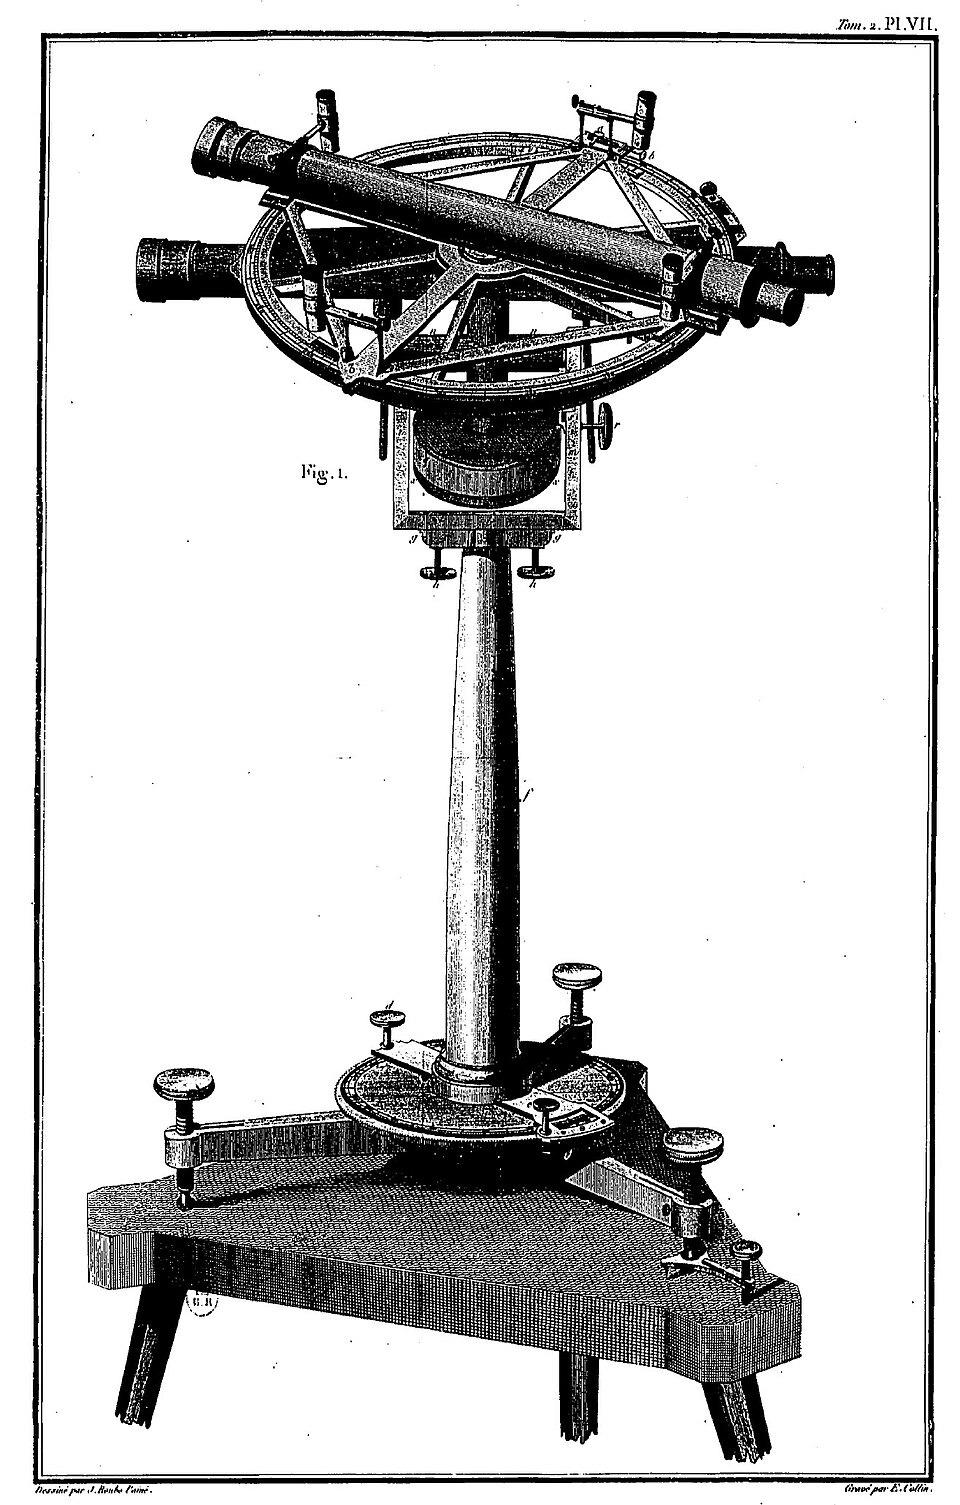
\includegraphics[width=0.3\linewidth]{images/book2/g10-delambre-repeating-circle.jpg}

{\small Um círculo repetidor montado para medir ângulos horizontais, como
gravado no relato de Delambre sobre a medição (1807). Domínio público
(Wikimedia Commons).}
\end{center}
\end{history}

\section{Uma Terra achatada}

Por volta de 1687, Isaac Newton argumentou, a partir da sua teoria da
gravitação, que uma Terra em rotação deve ser um esferoide achatado nos
polos e dilatado no equador. Medidas de graus do meridiano feitas pelos
astrônomos do Observatório de Paris pareciam dizer o contrário: uma Terra
alongada nos polos. A questão foi decidida medindo o comprimento de um grau
de latitude em lugares tão afastados quanto possível.
% ledger: figure:expeditions

\begin{omfigure}
\begin{tikzpicture}[font=\small, >={Stealth[length=2mm]}]
  \def\a{3.0} \def\b{2.3}
  \draw[black!35, densely dashed] (0,0) circle (\a);
  \fill[omDef!8] (0,0) ellipse ({\a} and {\b});
  \draw[omDef!70!black, thick] (0,0) ellipse ({\a} and {\b});
  \draw[black!50] (-3.4,0) -- (3.7,0);
  \draw[black!50] (0,-2.6) -- (0,3.3);
  \draw[<->, omThm!85!black] (0,-0.3) -- (\a,-0.3);
  \node[omThm!85!black, below] at (1.5,-0.3) {$a$};
  \draw[<->, omThm!85!black] (-0.3,0) -- (-0.3,\b);
  \node[omThm!85!black, left] at (-0.3,1.15) {$b$};
  \node[above right] at (0,\b) {N};
  \node[anchor=south east] at (3.0,-2.5) {};
  \node[anchor=west] at (3.7,0) {equador};
  % normal at t = 45 deg: P = (2.121, 1.626); crosses the equator at (0.874,0), the axis at (0,-1.14)
  \coordinate (P) at (2.121,1.626);
  \draw[omExo!85!black, thick] (P) -- ($(P)!1.35!(0.874,0)$);
  \draw[omExo!85!black, thick, ->] (P) -- ($(P)!-0.45!(0.874,0)$);
  \fill (P) circle (1.6pt);
  \node[anchor=west, align=left, font=\footnotesize] at (2.85,2.35) {vertical local\\(fio de prumo)};
  \draw[omExo!85!black] (1.45,0) arc (0:52.5:0.58);
  \node[omExo!85!black] at (1.62,0.32) {$\varphi$};
  \fill (0,0) circle (1.3pt);
  \node[anchor=north east, font=\footnotesize] at (0,0) {centro};
  \node[black!50, font=\footnotesize, anchor=south] at (-2.2,2.15) {esfera};
\end{tikzpicture}

{\small Uma Terra achatada, com o \omterm{def:g10:measuring-the-earth:ellipsoid}{achatamento} muito exagerado (o verdadeiro
é pequeno demais para ser visto nesta escala). A vertical de um lugar é
perpendicular à superfície; ela não aponta exatamente para o centro. A
latitude $\varphi$ do lugar é o ângulo entre a sua vertical e o plano do
equador.}
\end{omfigure}

A latitude é medida pelas estrelas: é o ângulo entre a vertical local e o
plano do equador. Numa Terra achatada, a superfície é menos curva perto dos
polos do que perto do equador. Onde a superfície é menos curva, é preciso
percorrer uma distância maior sobre ela para que a vertical gire um grau:
\emph{um grau de latitude é mais longo perto dos polos}.

\begin{history}[Lapônia e Peru]
% ledger: figure:expeditions, figure:degrees
Em 1735, a Academia de Ciências de Paris enviou uma expedição ao equador, na
província espanhola do Peru (hoje o Equador); ela trabalhou ali durante nove
anos, até 1744. Em 1736--1737, uma segunda expedição, chefiada por
Pierre-Louis Moreau de Maupertuis com o jovem matemático Alexis Clairaut,
mediu um grau do meridiano na Lapônia, perto do Círculo Polar Ártico. O
grau da Lapônia deu 57\,437 \emph{toesas} (a antiga unidade de comprimento;
cerca de \qty{111.95}{km}), e o grau do Peru apenas 56\,737 toesas: o grau
é mais longo perto do polo, e Newton tinha razão. Os dois números
implicavam um \omterm{def:g10:measuring-the-earth:ellipsoid}{achatamento} de cerca de $1/205$ --- grande demais, como
mostraram levantamentos posteriores, mas a questão do sinal estava
resolvida.
\end{history}

\begin{omfigure}
\begin{tikzpicture}
\begin{axis}[omrecord, width=0.82\linewidth, height=5.4cm, xmin=0, xmax=90,
  ymin=110.45, ymax=111.8, xlabel={latitude (\unit{\degree})},
  ylabel={comprimento de \qty{1}{\degree} de latitude (km)}, xtick={0,15,...,90},
  ytick={110.6,110.8,...,111.8}, yticklabel style={/pgf/number format/fixed, /pgf/number format/fixed zerofill, /pgf/number format/precision=1}]
\addplot[omDef!85!black, line width=1.1pt] table[x=lat_deg, y=deg_km] {figdata/out/grade-10-meridian_degree.dat};
\addplot[only marks, mark=*, mark size=1.8pt, omThm!85!black] coordinates {(0,110.574) (45,111.132) (66,111.507) (90,111.694)};
\node[anchor=south west, font=\footnotesize] at (axis cs:2,110.6) {110.57 km};
\node[anchor=north east, font=\footnotesize] at (axis cs:89,111.56) {111.69 km};
\node[anchor=north west, font=\footnotesize] at (axis cs:46,111.12) {111.13 km};
\node[anchor=south east, font=\footnotesize] at (axis cs:65,111.53) {111.51 km a \ang{66} (Lapônia)};
\end{axis}
\end{tikzpicture}

{\small O comprimento de um grau de latitude no \omterm{def:g10:measuring-the-earth:ellipsoid}{elipsoide de referência} da
\cref{def:g10:measuring-the-earth:ellipsoid}, do equador ao polo. Calculado
com o elipsoide WGS~84.}
\end{omfigure}

\begin{definition}[Elipsoide de referência e achatamento]\label{def:g10:measuring-the-earth:ellipsoid}
Um \emph{elipsoide de referência}\index{elipsoide de referencia@elipsoide de referência}
é a superfície obtida pela rotação de uma elipse em torno do seu eixo
menor, escolhida para se ajustar o mais possível à forma da Terra. O seu
\emph{raio equatorial} é $a$, o seu \emph{raio polar} é $b$, e o seu
\emph{achatamento}\index{achatamento} é
\[
  f = \frac{a-b}{a}.
\]
\end{definition}

\begin{proposition}[As dimensões da Terra]\label{prop:g10:measuring-the-earth:dimensions}
% ledger: wgs84:ellipsoid, earth:Req, earth:Rpol, earth:Rmean (lengths computed in figdata/grade-10/meridian_degree.py)
O \omterm{def:g10:measuring-the-earth:ellipsoid}{elipsoide de referência} usado no posicionamento por satélite (WGS~84) tem
\[
  a = \qty{6378.137}{km}, \qquad b = \qty{6356.752}{km}, \qquad
  f = \frac{1}{298.257}.
\]
O raio polar é \qty{21.4}{km} mais curto que o raio equatorial. O equador
mede \qty{40075}{km} e um meridiano, de polo a polo e de volta,
\qty{40008}{km}; o quarto de meridiano, do equador a um polo, mede
\qty{10001.966}{km}. Um grau de latitude mede \qty{110.574}{km} no equador
e \qty{111.694}{km} nos polos. Um grau de longitude mede \qty{111.32}{km}
no equador e diminui em direção aos polos aproximadamente como
$\cos \varphi$.
\end{proposition}

\begin{example}[Um grau de longitude]\label{ex:g10:measuring-the-earth:longitude}
Um paralelo de latitude $\varphi$ é um círculo cujo raio é a distância ao
eixo, cerca de $R \cos \varphi$. A \qty{60}{\degree} N, a sua circunferência
é cerca de metade da do equador, e um grau de longitude mede cerca de
$111.32 \times \cos 60^\circ \approx \qty{55.7}{km}$ (o elipsoide dá
\qty{55.80}{km}).
\end{example}

\begin{remark}[Quão redonda é a Terra?]\label{rem:g10:measuring-the-earth:round}
Um \omterm{def:g10:measuring-the-earth:ellipsoid}{achatamento} de $1/298$ é pequeno. Num globo de \qty{30}{cm} de diâmetro,
o diâmetro polar seria apenas \qty{1}{mm} mais curto que o equatorial ---
invisível. A fossa oceânica mais profunda, a quase \qty{11}{km} abaixo do
nível do mar, seria um arranhão de cerca de um quarto de milímetro de
profundidade. Para a maioria dos usos, a Terra é uma esfera de raio médio
\qty{6371}{km}; para posições precisas, é preciso o elipsoide.
% ledger: earth:Rmean, usgs:trench-depth
\end{remark}

\section{A geodésia hoje}

\begin{omfigure}
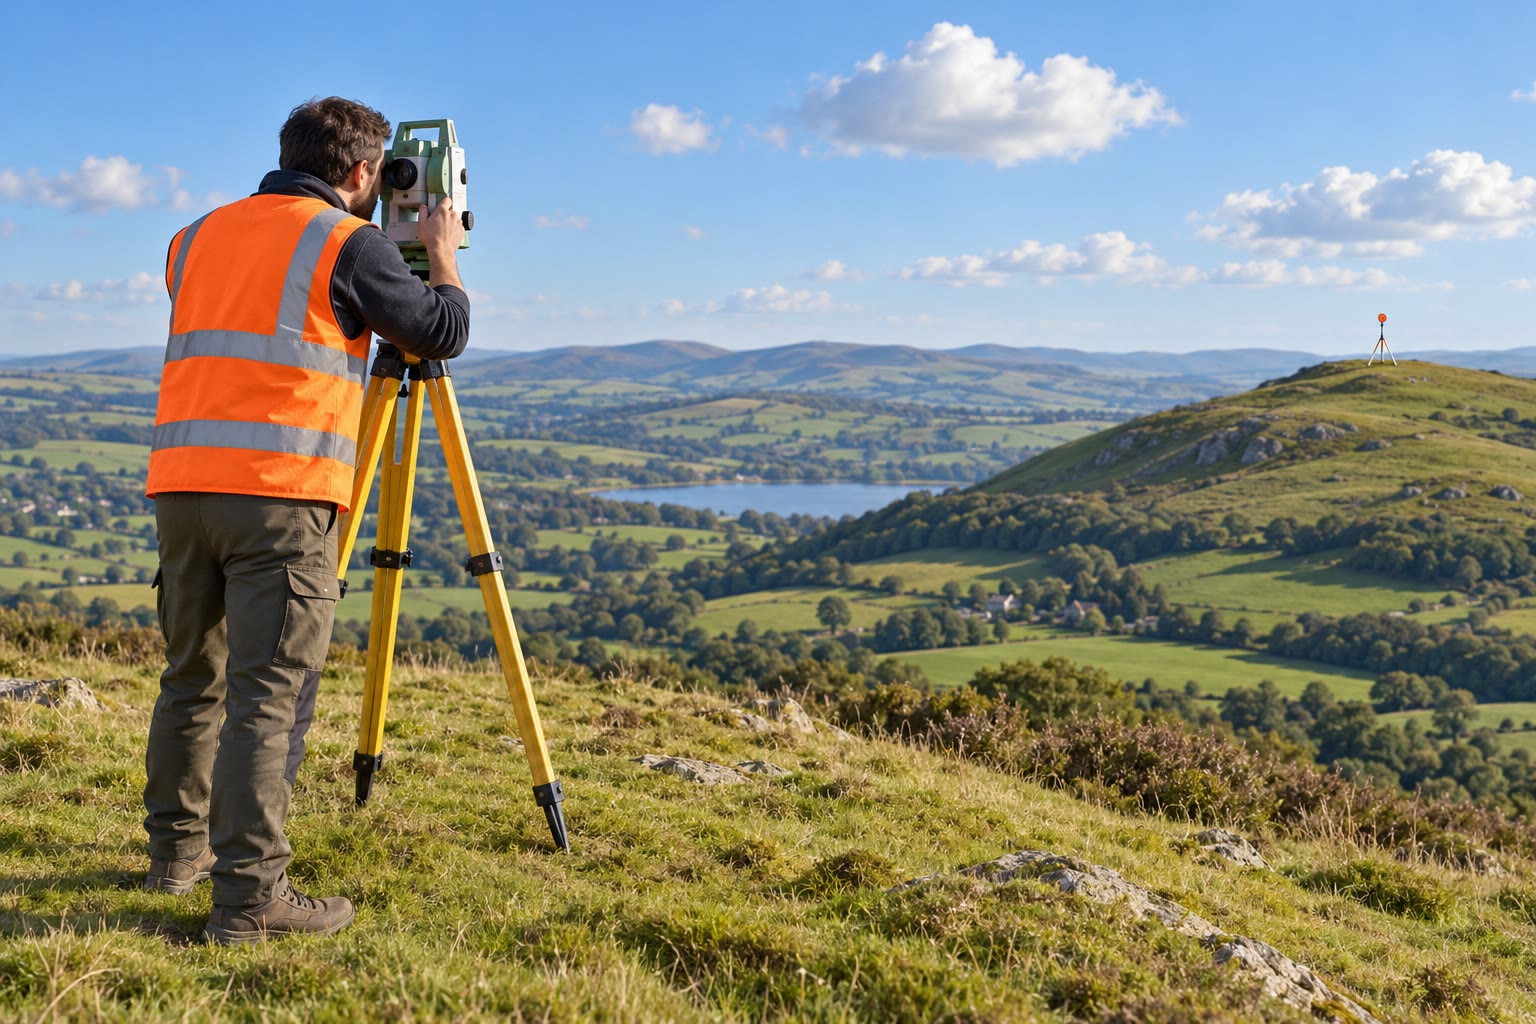
\includegraphics[width=0.7\linewidth]{images/book2/ai/g10-surveyor-theodolite.jpg}

{\small Um agrimensor trabalhando com um instrumento moderno que mede
ângulos e, com um feixe de luz, distâncias; um sinal de levantamento está
plantado no morro ao fundo.}
\end{omfigure}

As grandes triangulações dos séculos~XVIII e XIX foram substituídas pelos
satélites. Um receptor no chão capta os sinais de vários satélites cujas
posições são conhecidas a cada instante e calcula a sua própria posição a
partir dos tempos de percurso dos sinais (Livro 1). Redes de receptores
permanentes, fixados no substrato rochoso no mundo inteiro, medem as suas
posições continuamente. Elas definem o referencial em que todo mapa e toda
posição por satélite são dados, e elas se movem: mostram as placas da
litosfera derivando alguns centímetros por ano
(\cref{ch:g11:plate-motions}).
% ledger: usgs:gps

\begin{inthefield}[Medir o terreno hoje]
Os geodesistas fixam antenas em pilares de concreto assentados no
substrato rochoso, longe de prédios e árvores, e registram as suas
posições a cada poucos segundos durante anos. Eles combinam esses dados
com medidas de radiotelescópios que observam galáxias muito distantes e
com feixes de laser disparados contra satélites que levam espelhos. Os
agrimensores, nos canteiros de obras e no campo, ainda medem ângulos e
distâncias com instrumentos sobre tripés, e os amarram ao referencial dos
satélites.
\end{inthefield}

\section{Exercícios}

\begin{exercise}[$\star$]\label{exo:g10:measuring-the-earth:1}
Dê três observações, possíveis sem sair do chão, que mostram que a Terra é
redonda. Para cada uma, explique numa frase por que uma Terra plana não
poderia produzi-la.
\end{exercise}

\begin{exercise}[$\star$]\label{exo:g10:measuring-the-earth:2}
O que é a \omterm{def:g10:measuring-the-earth:geodesy}{geodésia}? O que é a \omterm{def:g10:measuring-the-earth:triangulation}{triangulação}, e qual é o único comprimento
que precisa ser medido no chão numa \omterm{def:g10:measuring-the-earth:triangulation}{triangulação}?
\end{exercise}

\begin{exercise}[$\star$]\label{exo:g10:measuring-the-earth:3}
Eratóstenes verificou que o ângulo entre os raios do Sol e a vertical em
Alexandria era $1/50$ de volta completa quando o Sol estava a pino em
Siena, a 5000 estádios dali. Calcule a circunferência em estádios e depois
em quilômetros, tomando um estádio de \qty{157.2}{m}.
\end{exercise}

\begin{exercise}[$\star$]\label{exo:g10:measuring-the-earth:4}
Um grau de latitude mede cerca de \qty{111}{km}. Quanto mede um minuto de
latitude ($1/60$ de grau)? Quanto mede, aproximadamente, o meridiano do
equador ao polo?
\end{exercise}

\begin{exercise}[$\star$]\label{exo:g10:measuring-the-earth:5}
Usando o raio equatorial \qty{6378.137}{km} e o raio polar
\qty{6356.752}{km}, calcule a diferença dos dois raios e o \omterm{def:g10:measuring-the-earth:ellipsoid}{achatamento}
$f = (a-b)/a$. Escreva $f$ como um dividido por um número inteiro.
\end{exercise}

\begin{exercise}[$\star\star$]\label{exo:g10:measuring-the-earth:6}
Duas cidades estão no mesmo meridiano, a \qty{500}{km} uma da outra. Ao
meio-dia do mesmo dia, uma vara vertical de \qty{1.00}{m} de altura projeta
uma sombra de \qty{0.364}{m} na cidade do sul e de \qty{0.456}{m} na
cidade do norte. Calcule o ângulo entre os raios do Sol e a vertical em
cada cidade e, depois, a circunferência da Terra.
\end{exercise}

\begin{exercise}[$\star\star$]\label{exo:g10:measuring-the-earth:7}
Num triângulo $ABC$, a base $AB = \qty{10.00}{km}$, o ângulo em $A$ é de
\qty{62}{\degree} e o ângulo em $B$ é de \qty{71}{\degree}. Calcule o
ângulo em $C$ e os comprimentos $AC$ e $BC$.
\end{exercise}

\begin{exercise}[$\star\star$]\label{exo:g10:measuring-the-earth:8}
Um avião voa exatamente para oeste ao longo do paralelo \qty{60}{\degree} N,
da longitude \qty{10}{\degree} L à longitude \qty{20}{\degree} O. Usando um
grau de longitude de $111.3 \cos \varphi$ km, calcule a distância que ele
percorre. Quanto mediria a mesma variação de longitude sobre o equador?
\end{exercise}

\begin{exercise}[$\star\star$]\label{exo:g10:measuring-the-earth:9}
O olho de um observador está a $h = \qty{2}{m}$ acima de um mar calmo. A
linha de visada até o horizonte tangencia o mar em $T$; o centro da Terra é
$O$, e o olho, $E$. Explique por que o triângulo $OTE$ tem um ângulo reto
em $T$ e, depois, use o teorema de Pitágoras com $R = \qty{6371}{km}$ para
mostrar que a distância até o horizonte é de cerca de $\sqrt{2Rh}$, e
calcule-a.
\end{exercise}

\begin{exercise}[$\star\star$]\label{exo:g10:measuring-the-earth:10}
Leia a curva dos comprimentos de grau. Entre quais latitudes o comprimento
de um grau varia mais depressa? Explique em duas frases por que um grau de
latitude é mais longo perto dos polos do que perto do equador.
\end{exercise}

\begin{exercise}[$\star\star$]\label{exo:g10:measuring-the-earth:11}
O arco de meridiano de Dunquerque a Barcelona abrange \qty{9.646}{\degree}
de latitude e mede \qty{1072.2}{km}. Calcule o comprimento médio de um grau
ao longo dele. Se todos os graus tivessem esse comprimento, quanto mediria
o quarto de meridiano? Compare com \qty{10002.0}{km} e explique a pequena
diferença.
\end{exercise}

\begin{exercise}[$\star\star\star$]\label{exo:g10:measuring-the-earth:12}
Eratóstenes mediu um ângulo de \qty{7.2}{\degree} e uma distância de 5000
estádios. Se o seu ângulo estivesse errado em \qty{0.1}{\degree} (pequeno
demais), em que porcentagem a sua circunferência estaria errada, e em que
sentido? Qual das suas duas medidas você acha que era a menos precisa?
\end{exercise}

\begin{exercise}[$\star\star\star$]\label{exo:g10:measuring-the-earth:13}
Uma cadeia de dois triângulos: em $ABC$, $AB = \qty{6.000}{km}$,
$A = \qty{55}{\degree}$, $B = \qty{75}{\degree}$. No triângulo seguinte,
$ACD$, construído sobre o lado $AC$, o ângulo em $A$ é de
\qty{50}{\degree} e o ângulo em $C$ é de \qty{68}{\degree}. Calcule $AC$
e, depois, $AD$.
\end{exercise}

\begin{exercise}[$\star\star\star$]\label{exo:g10:measuring-the-earth:14}
Em que latitude um grau de longitude mede a metade do que mede no equador?
Em que latitude ele mede um décimo? Explique por que nenhuma das duas
respostas depende do tamanho da Terra.
\end{exercise}

\begin{exercise}[$\star\star\star$]\label{exo:g10:measuring-the-earth:15}
Use os valores do elipsoide: um grau de latitude mede \qty{110.574}{km} no
equador e \qty{111.694}{km} no polo. Numa esfera de mesmo raio médio, um
grau mediria \qty{111.195}{km} em toda parte. Em quantos metros erraria um
agrimensor que supusesse uma esfera, ao longo de um grau no equador e ao
longo de um grau no polo? Por que um mapa que dá posições com precisão de
um metro precisa ser calculado sobre o elipsoide?
\end{exercise}

\section{Problema: o metro e o meridiano}

\begin{problem}[{Problema de fim de semana --- da sombra de Eratóstenes ao
comprimento do primeiro metro}]
\label{pb:g10:measuring-the-earth:1}
% ledger: geonames:aswan, geonames:alexandria, erat:method, metre:1791, metre:survey, wgs84:ellipsoid (arc lengths and degree lengths computed in figdata/grade-10/meridian_degree.py)
Um estudante refaz a história da medida da Terra com números modernos.
Assuã, a antiga Siena, fica na latitude \qty{24.09}{\degree} N, e
Alexandria a \qty{31.20}{\degree} N; no elipsoide moderno, o arco de
meridiano entre os seus dois paralelos mede \qty{788}{km}. No elipsoide, um
grau de latitude mede \qty{110.57}{km} no equador, \qty{111.13}{km} a
\qty{45}{\degree} e \qty{111.51}{km} a \qty{66}{\degree}, e o quarto de
meridiano mede \qty{10001.966}{km}.

\medskip
\noindent\textbf{Parte I --- Eratóstenes de novo.}
\begin{enumerate}
  \item Calcule a diferença de latitude entre Assuã e Alexandria.
  \item Que fração de uma volta completa ela representa? Compare com o
        $1/50$ de Eratóstenes.
  \item Calcule a circunferência da Terra que o método de Eratóstenes dá
        com esses números modernos.
  \item As duas cidades não estão no mesmo meridiano: Assuã fica cerca de
        \qty{3}{\degree} de longitude a leste de Alexandria. Que distância
        deve ser usada no método: a distância em linha reta entre as
        cidades ou o arco de meridiano entre os seus paralelos? Por quê?
  \item Por que as duas sombras precisam ser medidas no mesmo dia, ao
        meio-dia solar local?
\end{enumerate}

\medskip
\noindent\textbf{Parte II --- Uma pequena triangulação.}
Mede-se uma base $AB = \qty{12.000}{km}$. De $A$, o sinal $C$ é visto a
\qty{58}{\degree} de $B$; de $B$, a \qty{66}{\degree} de $A$. No triângulo
seguinte, $ACD$, o ângulo em $A$ é de \qty{47}{\degree} e o ângulo em $C$
é de \qty{75}{\degree}. O lado $AD$ aponta \qty{8}{\degree} a leste do
norte.
\begin{enumerate}[resume]
  \item Calcule o ângulo em $C$ no triângulo $ABC$.
  \item Calcule o lado $AC$.
  \item Calcule o lado $BC$.
  \item Calcule o ângulo em $D$ no triângulo $ACD$ e, depois, o lado $AD$.
  \item Calcule a distância norte--sul entre $A$ e $D$.
  \item Usando o comprimento do grau a \qty{45}{\degree}, calcule a
        diferença de latitude entre $A$ e $D$, em graus e em minutos de
        arco.
\end{enumerate}

\medskip
\noindent\textbf{Parte III --- Uma Terra achatada.}
\begin{enumerate}[resume]
  \item Em quantos metros um grau de latitude a \qty{66}{\degree} é mais
        longo que um grau no equador?
  \item Explique o que essa diferença mostra sobre a forma da Terra.
  \item No elipsoide, $a = \qty{6378.137}{km}$ e
        $b = \qty{6356.752}{km}$. Calcule $a - b$ e o \omterm{def:g10:measuring-the-earth:ellipsoid}{achatamento}.
  \item Explique por que, numa Terra achatada, o fio de prumo num lugar de
        latitude \qty{45}{\degree} não aponta exatamente para o centro da
        Terra.
\end{enumerate}

\medskip
\noindent\textbf{Parte IV --- O primeiro metro.}
\begin{enumerate}[resume]
  \item Segundo a definição de 1791, quanto deveria medir o quarto de
        meridiano, em metros?
  \item O metro de platina de 1799 foi fabricado a partir de um valor
        medido do meridiano. Se o quarto de meridiano mede na verdade
        \qty{10001.966}{km}, quanto mede a sua décima milionésima parte?
  \item O metro de 1799 era longo ou curto demais em relação à sua própria
        definição? Em que fração?
  \item A barra de platina copiou fielmente o comprimento calculado nos
        anos 1790. O quarto de meridiano calculado naquela época era longo
        ou curto demais? Explique.
  \item Em quantos milímetros o primeiro metro era mais curto que a décima
        milionésima parte do verdadeiro quarto de meridiano? Compare com a
        espessura de uma folha de papel, cerca de \qty{0.1}{mm}.
\end{enumerate}
\end{problem}
